\documentclass[a4paper, titlepage]{article}
\usepackage[round, sort, numbers]{natbib}
\usepackage[utf8]{inputenc}
\usepackage{amsfonts, amsmath, amssymb, amsthm}
\usepackage{color}
\usepackage{listings}
\usepackage{mathtools}
\usepackage{paralist}
\usepackage{parskip}
\usepackage{subfig}
\usepackage{tikz}
\usepackage{titlesec}

\numberwithin{figure}{section}
\numberwithin{table}{section}

\usetikzlibrary{arrows, automata, backgrounds, petri, positioning}
\tikzstyle{place}=[circle, draw=blue!50, fill=blue!20, thick]
\tikzstyle{transition}=[rectangle, draw=black!50, fill=black!20, thick]

% define new commands for sets and tuple
\newcommand{\setof}[1]{\ensuremath{\left \{ #1 \right \}}}
\newcommand{\tuple}[1]{\ensuremath{\left \langle #1 \right \rangle }}
\newcommand{\card}[1]{\ensuremath{\left \vert #1 \right \vert }}

\makeatletter
\newcommand\objective[1]{\def\@objective{#1}}
\newcommand{\makecustomtitle}{%
	\begin{center}
		\huge\@title \\
		[1ex]\small Dimitri Racordon \\ \@date
	\end{center}
	\@objective
}
\makeatother

\begin{document}

  \title{Outils formels de Modélisation \\ 3\textsuperscript{ème} séance d'exercices}
  \author{Dimitri Racordon}
  \date{07.10.16}
  \objective{
    Dans cette séance d'exercices,
    nous allons manipuler des propriétés inhérentes aux réseaux de Petri.
    Nous étudierons la signification de ces propriétés par l'exemple
    avant des les exprimer formellement.
  }

	\makecustomtitle

  \section{Graphe de marquage ($\bigstar$)}
		Considérez le réseau de Petri de la figure \ref{fig:exclusion},
    représentant une exclusion mutuelle.
    Créez le graphe de marquage de ce réseau et répondez aux questions suivantes:
		\begin{enumerate}
			\item Quelles sont les propriétés que vous pouvez déduire du graphe de marquage?
			\item Que signifient ces propriétés en relation avec le système modélisé.
		\end{enumerate}

		Modifiez le marquage initial en ajoutant 1 jeton dans la place $r_0$
    et recréez son graphe de marquage.

		\begin{enumerate}
			\item Combien de noeuds comporte le nouveau graphe de marquage?
			\item Si on augmente encore le nombre de jetons dans la place $r_0$,
            cela aura-t-il un impact sur le nombre de noeuds du graphe de marquage?
		\end{enumerate}

		\begin{figure}[ht]
			\centering
      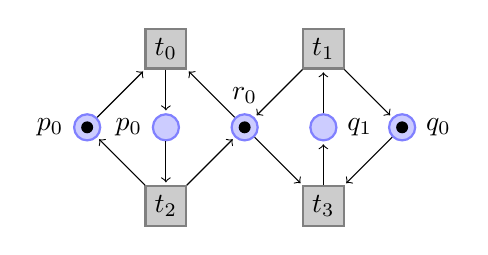
\begin{tikzpicture}
        \node[place,tokens=1] (p0) [label=left:$p_0$] {};
        \node[place] (p1) [right of=p0, label=left:$p_0$] {};
        \node[place,tokens=1] (r0) [right of=p1, label=above:$r_0$] {};
        \node[place] (q1) [right of=r0, label=right:$q_1$] {};
        \node[place,tokens=1] (q0) [right of=q1, label=right:$q_0$] {};

        \node [transition] (t0) [above of=p1] {$t_0$}
						  edge [pre] (p0) edge [pre] (r0)
							edge [post] (p1);
        \node [transition] (t1) [above of=q1] {$t_1$}
						  edge [pre] (q1)
							edge [post] (r0) edge [post] (q0);
        \node [transition] (t2) [below of=p1] {$t_2$}
						  edge [pre] (p1)
							edge [post] (r0) edge [post] (p0);
        \node [transition] (t3) [below of=q1] {$t_3$}
						  edge [pre] (q0) edge [pre] (r0)
							edge [post] (q1);
      \end{tikzpicture}
			\caption{Un modèle Smith}
			\label{fig:exclusion}
		\end{figure}

  \section{A trois on tire ($\bigstar\bigstar$)}
    Considérez le réseau de la figure \ref{fig:sequence} et répondez aux questions suivantes:
    \begin{enumerate}
      \item Encodez ce réseau en Swift à l'aide de la librarie PetriKit.
      \item Ecrivez une séquence de transitions $s$
            telle que $M_0 \rightarrow_s$ laisse le réseau bloqué.
            Existe-t-il une seule séquence avec cette propriété?
      \item Ecrivez le maquage initial minimal $M_0$
            permettant de tirer la séquence
            $t_0 \rightarrow t_2 \rightarrow t_1 \rightarrow t_2 \rightarrow t_0$.
    \end{enumerate}

  \begin{figure}[ht]
    \centering
    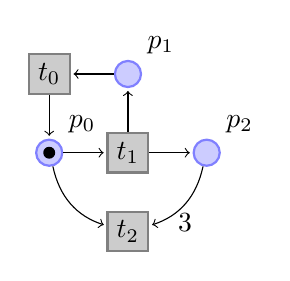
\begin{tikzpicture}
      \node[place,tokens=1] (p0) [label=45:$p_0$] {};
      \node[place] (p1) [right of=p0, yshift=1cm, label=45:$p_1$] {};
      \node[place] (p2) [right of=p0, xshift=1cm, label=45:$p_2$] {};

      \node [transition] (t0) [above of=p0] {$t_0$}
            edge [pre] (p1)
            edge [post] (p0);
      \node [transition] (t1) [right of=p0] {$t_1$}
            edge [pre] (p0)
            edge [post] (p1) edge [post] (p2);
      \node [transition] (t2) [below of=t1] {$t_2$}
            edge [pre, bend left] (p0) edge [pre, bend right] node[below] {3} (p2);
    \end{tikzpicture}
    \caption{Un réseau de Petri}
    \label{fig:sequence}
  \end{figure}

  \section{Définition formelle de propriétés ($\bigstar\bigstar$)}
		Définissez formellement les propriétés suivantes, \textbf{puis} créez un exemple de réseau de Petri les illustrant:
		\begin{enumerate}
			\item Un réseau de Petri où au plus une place est vide, et ce pour tous les marquages atteignables.
			\item Un réseau de Petri dont le nombre de jeton dans chaque place est borné à 42.
			\item Un réseau de Petri dont aucune transition n'est vivante.
		\end{enumerate}

\end{document}
